\addtocontents{toc}{\protect\vspace{30pt}}

\chapter{Liste der implementierten Klassen und Methoden}
\label{appendix:classes}
\section{dll.py}

\begin{itemize}

    \item \texttt{Leaf}: Ein Element einer doppelt verketteten List mit den Attributen \texttt{key}, \texttt{value}, \texttt{prev} und \texttt{succ}

    \begin{itemize}
        \item \texttt{insertAfter}: Fügt ein Objekt nach dem Objekt ein
        \item \texttt{insertBefore}: Fügt ein Objekt vor dem Objekt ein
        \item \texttt{remove}: Entfernt das Objekt
    \end{itemize}

    \item \texttt{DoublyLinkedList}: Eine doppelt verkettete Liste, enthält die Referenz zum Dummy Element mit dem Schlüssel $\infty$.

    \begin{itemize}
        \item \texttt{locate}: Findet das Element mit dem gesuchten Schlüssel.
        \item \texttt{insert}: Fügt ein Element mit dem gegebenen Schlüssel ein.
        \item \texttt{remove}: Entfernt das Element mit dem gegebenen Schlüssel.
        \item \texttt{isEmpty}: Prüft Liste auf Leere.
        \item \texttt{first}: Gibt erstes Element zurück.
        \item \texttt{last}: Gibt letztes Element zurück.
        \item \texttt{count}: Gibt Anzahl der Elemente in der Liste zurück.
        \item \texttt{listAll}: Gibt alle Elemente der Reihenfolge nach auf der Kommandozeile aus.
    \end{itemize}

\end{itemize}

\section{abTree.py}

\begin{itemize}

    \item \texttt{Node}: Ein Knotenpunkt in einem (a,b)-Baum, enthält die Attribute \texttt{s} (Liste von Teilerschlüsseln), \texttt{c} (Liste von Referenzen zu Unterknotenpunkten oder Blättern) und \texttt{d} (Der Grad des Knotenpunktes).

    \begin{itemize}
        \item \texttt{locateLocally}: Lokalisiert einen Teilerschlüssel innerhalb eines Knotenpunktes.
        \item \texttt{getMax}: Gibt das letzte Element im Unterbaum des Knotenpunktes zurück, ohne die doppelt verkettete Liste zu benutzen.
        \item \texttt{locateRec}: Gibt das Element mit dem gegebenen Schlüssel zurück, insofern es in der Sequenz vorhanden ist. Wenn nicht, gibt es das nächstgrößere Element zurück.
        \item \texttt{insertRec}: Fügt ein Element mit dem gegebenen Schlüssel an der richtigen Stelle im Unterbaum des Knotenpunktes ein.
        \item \texttt{removeLocally}: Entfernt ein Kind mit dem gegebenen Index vom Knotenpunkt.
        \item \texttt{removeRec}: Entfernt das Element mit dem gegebenen Schlüssel aus dem Unterbaum des Knotenpunktes.
        \item \texttt{mergeRec}: Fügt einen Unterbaum an den aktuellen Knotenpunkt an. Es muss angegeben werden, ob dies auf der linken oder rechten Seite erfolgen soll. Des Weiteren muss die Differenz der Höhen der zwei Bäume angegeben werden.
        \item \texttt{splitRec}: Teilt den Baum ausgehend vom Knotenpunkt in zwei Hälften, eine links vom gegebenen Schlüssel, und eine rechts  davon.
    \end{itemize}

    \item \texttt{ABTree}: Ein (a,b)-Baum, enthält die Attribute \texttt{root} (Wurzel-Knotenpunkt), \texttt{list} (die dazugehörige doppelt verkettete Liste) und \texttt{height} (Die Höhe des Baumes).

    \begin{itemize}
        \item \texttt{locate}: Gibt das Element mit dem angegeben Schlüssel zurück, falls es exisiteirt. Wenn nicht, wird das nächste Element zurückgegeben.
        \item \texttt{insert}: Fügt ein Element mit dem gegebenen Schlüssel an der richtigen Stelle des Baumes ein.
        \item \texttt{remove}: Entfernt das Element mit dem gegebenen Schlüssel, insofern es existiert.
        \item \texttt{listAll}: Führt \texttt{listAll} der Liste des Baumes aus.
        \item \texttt{count}: Führt \texttt{count} der Liste des Baumes aus.
        \item \texttt{first}: Führt \texttt{first} der Liste des Baumes aus.
        \item \texttt{last}: Führt \texttt{last} der Liste des Baumes aus.
        \item \texttt{isEmpty}: Führt \texttt{isEmpty} der Liste des Baumes aus.
        \item \texttt{locateRange}: Gibt alle Elemente innerhalb des gegebenen Bereiches zurück (als Liste).
        \item \texttt{split}: Teilt den Baum in zwei Unterbäume, die Teilung erfolgt am Element mit dem angegebenen Schlüssel, oder am nächstgrößeren, falls es nicht in der Liste vorhanden ist.
        \item \texttt{bulkInsert}: Fügt mehrere Elemente auf einmal ein, in parallelen Prozessen (nicht funktionstüchtig)
    \end{itemize}

    \item \texttt{mergeTrees}: Fügt zwei Bäume zu einem zusammen. Sie dürfen sich nicht überschneiden.

\end{itemize}

\chapter{weitere Testergebnisse}
\label{appendix:benchmarks}

\vskip 4cm

\begin{figure}[hbt!]
    \centering{
        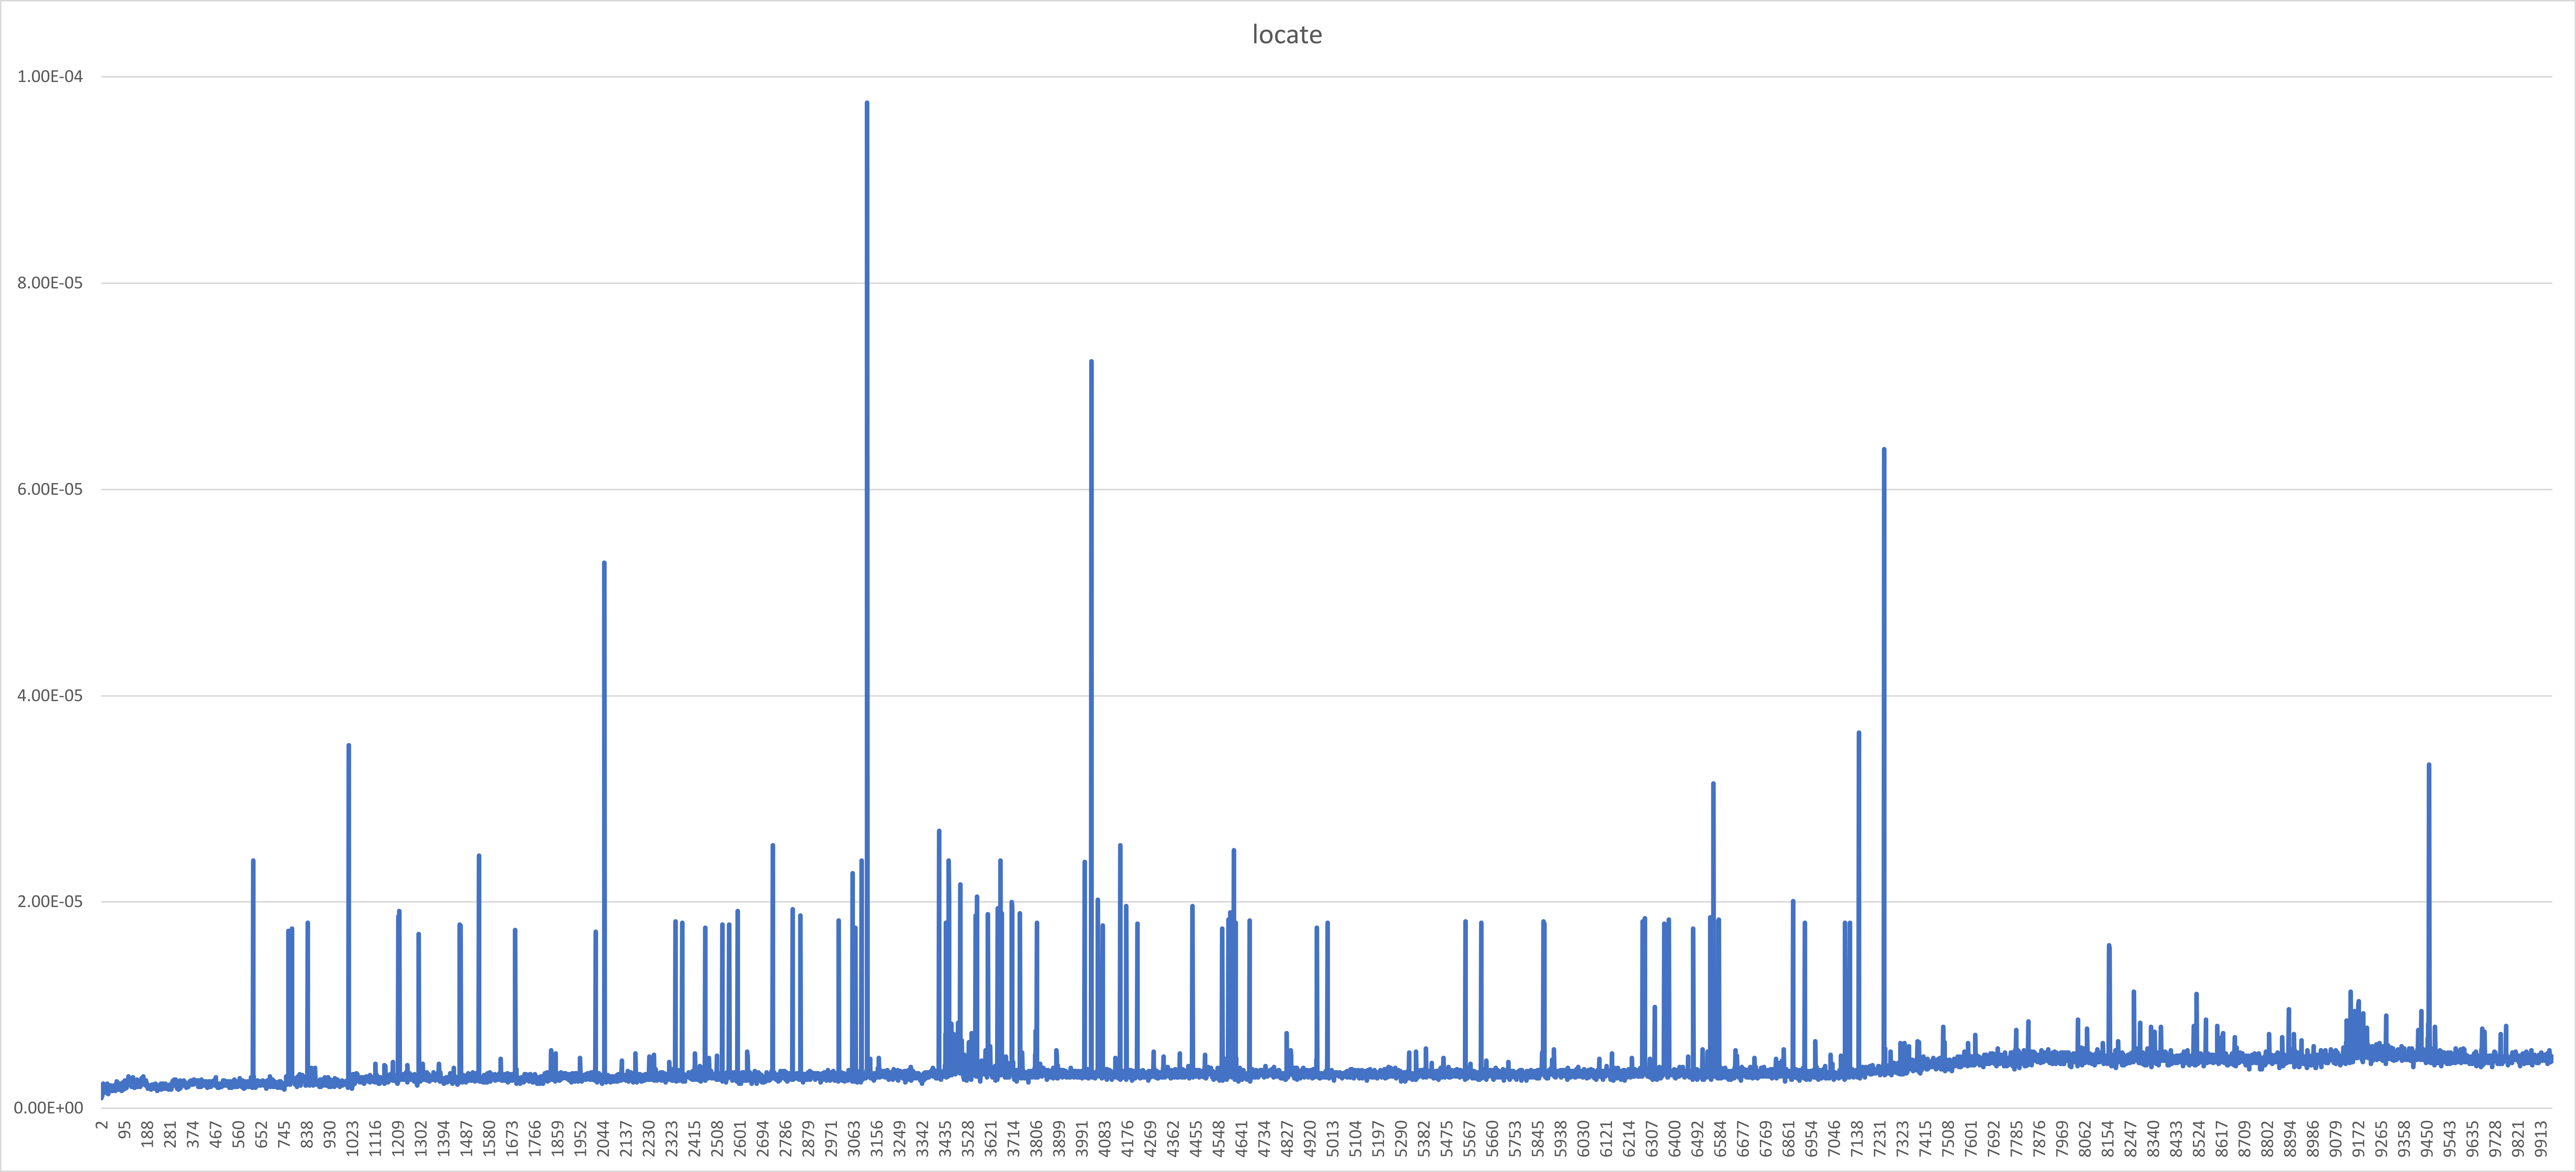
\includegraphics[width=\linewidth]{assets/benchmark10raw.png}
        \caption{Die unbearbeiteten Ergebnisse des Tests an einer sortierten Sequenz mit maximal 10.000 Elementen. Dargestellt ist die Dauer der Funktion \texttt{locate}. Durch die großen Messspitzen sind die Ergebnisse nicht gut ablesbar.}
        \label{fig:benchmark10raw}
    }
\end{figure}

\begin{figure}
    \centering{
        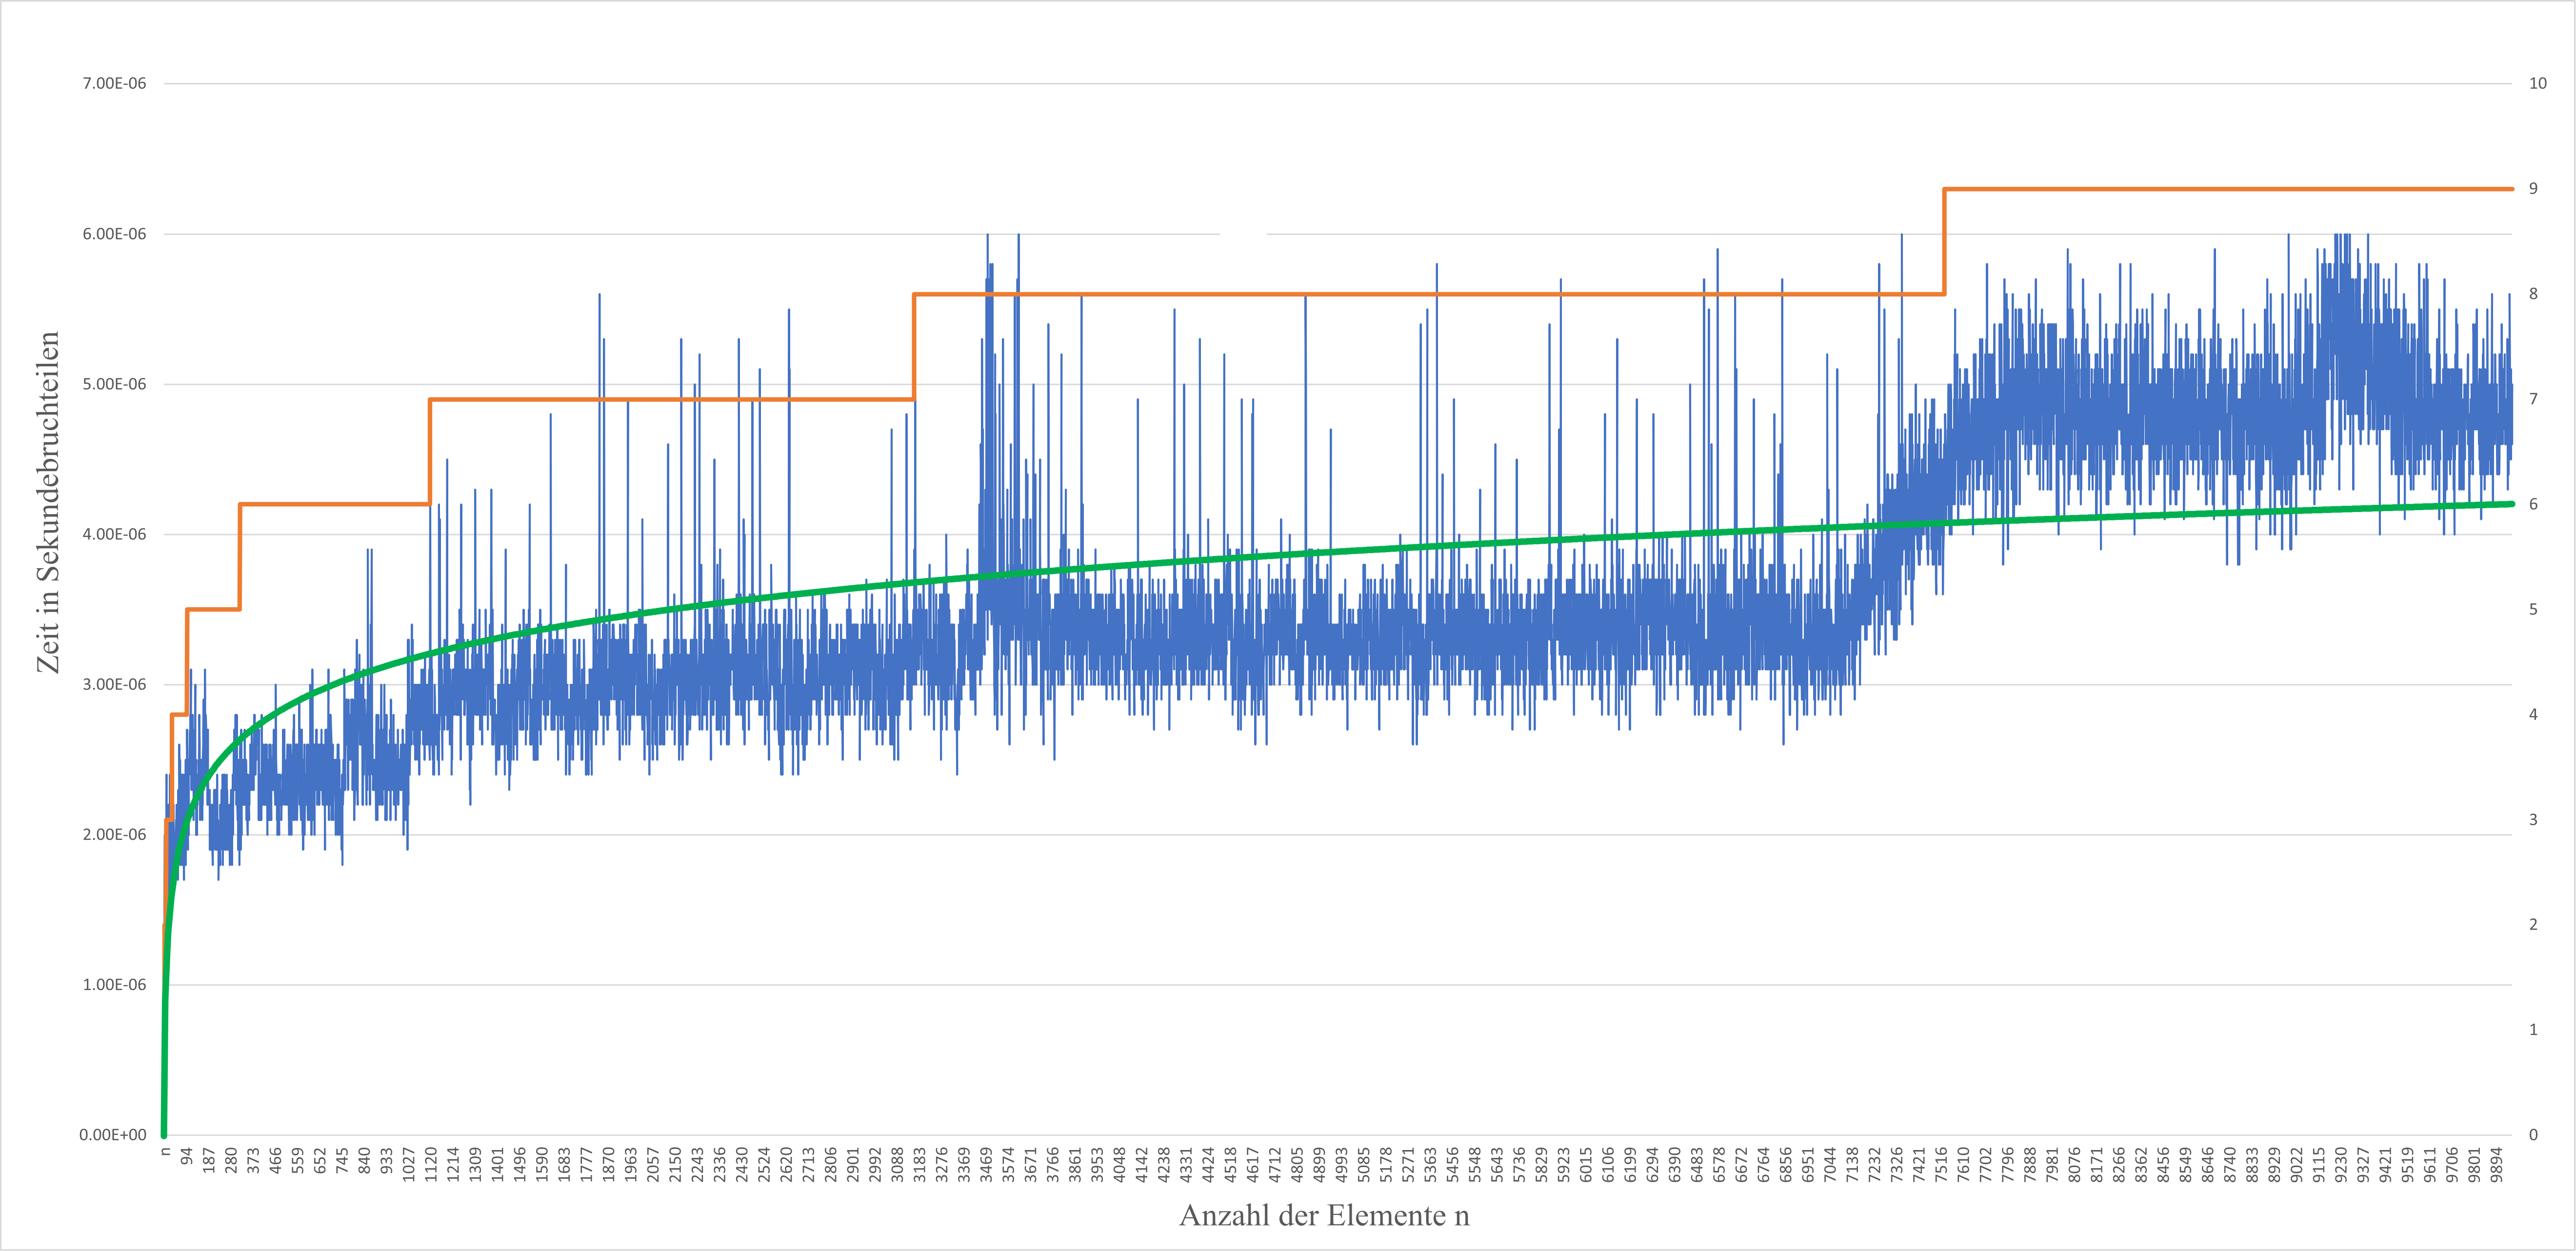
\includegraphics[width=\linewidth]{assets/benchmark10.png}
        \caption{Die bearbeiteten Ergebnisse des Testes mit 10.000 Elementen zeigen die logarithmische Laufzeit von \texttt{locate}, sowie die Abhängigkeit von der Höhe des Baumes (orange dargestellt)}
        \label{fig:benchmark10}
    }
\end{figure}

\begin{figure}
    \centering{
        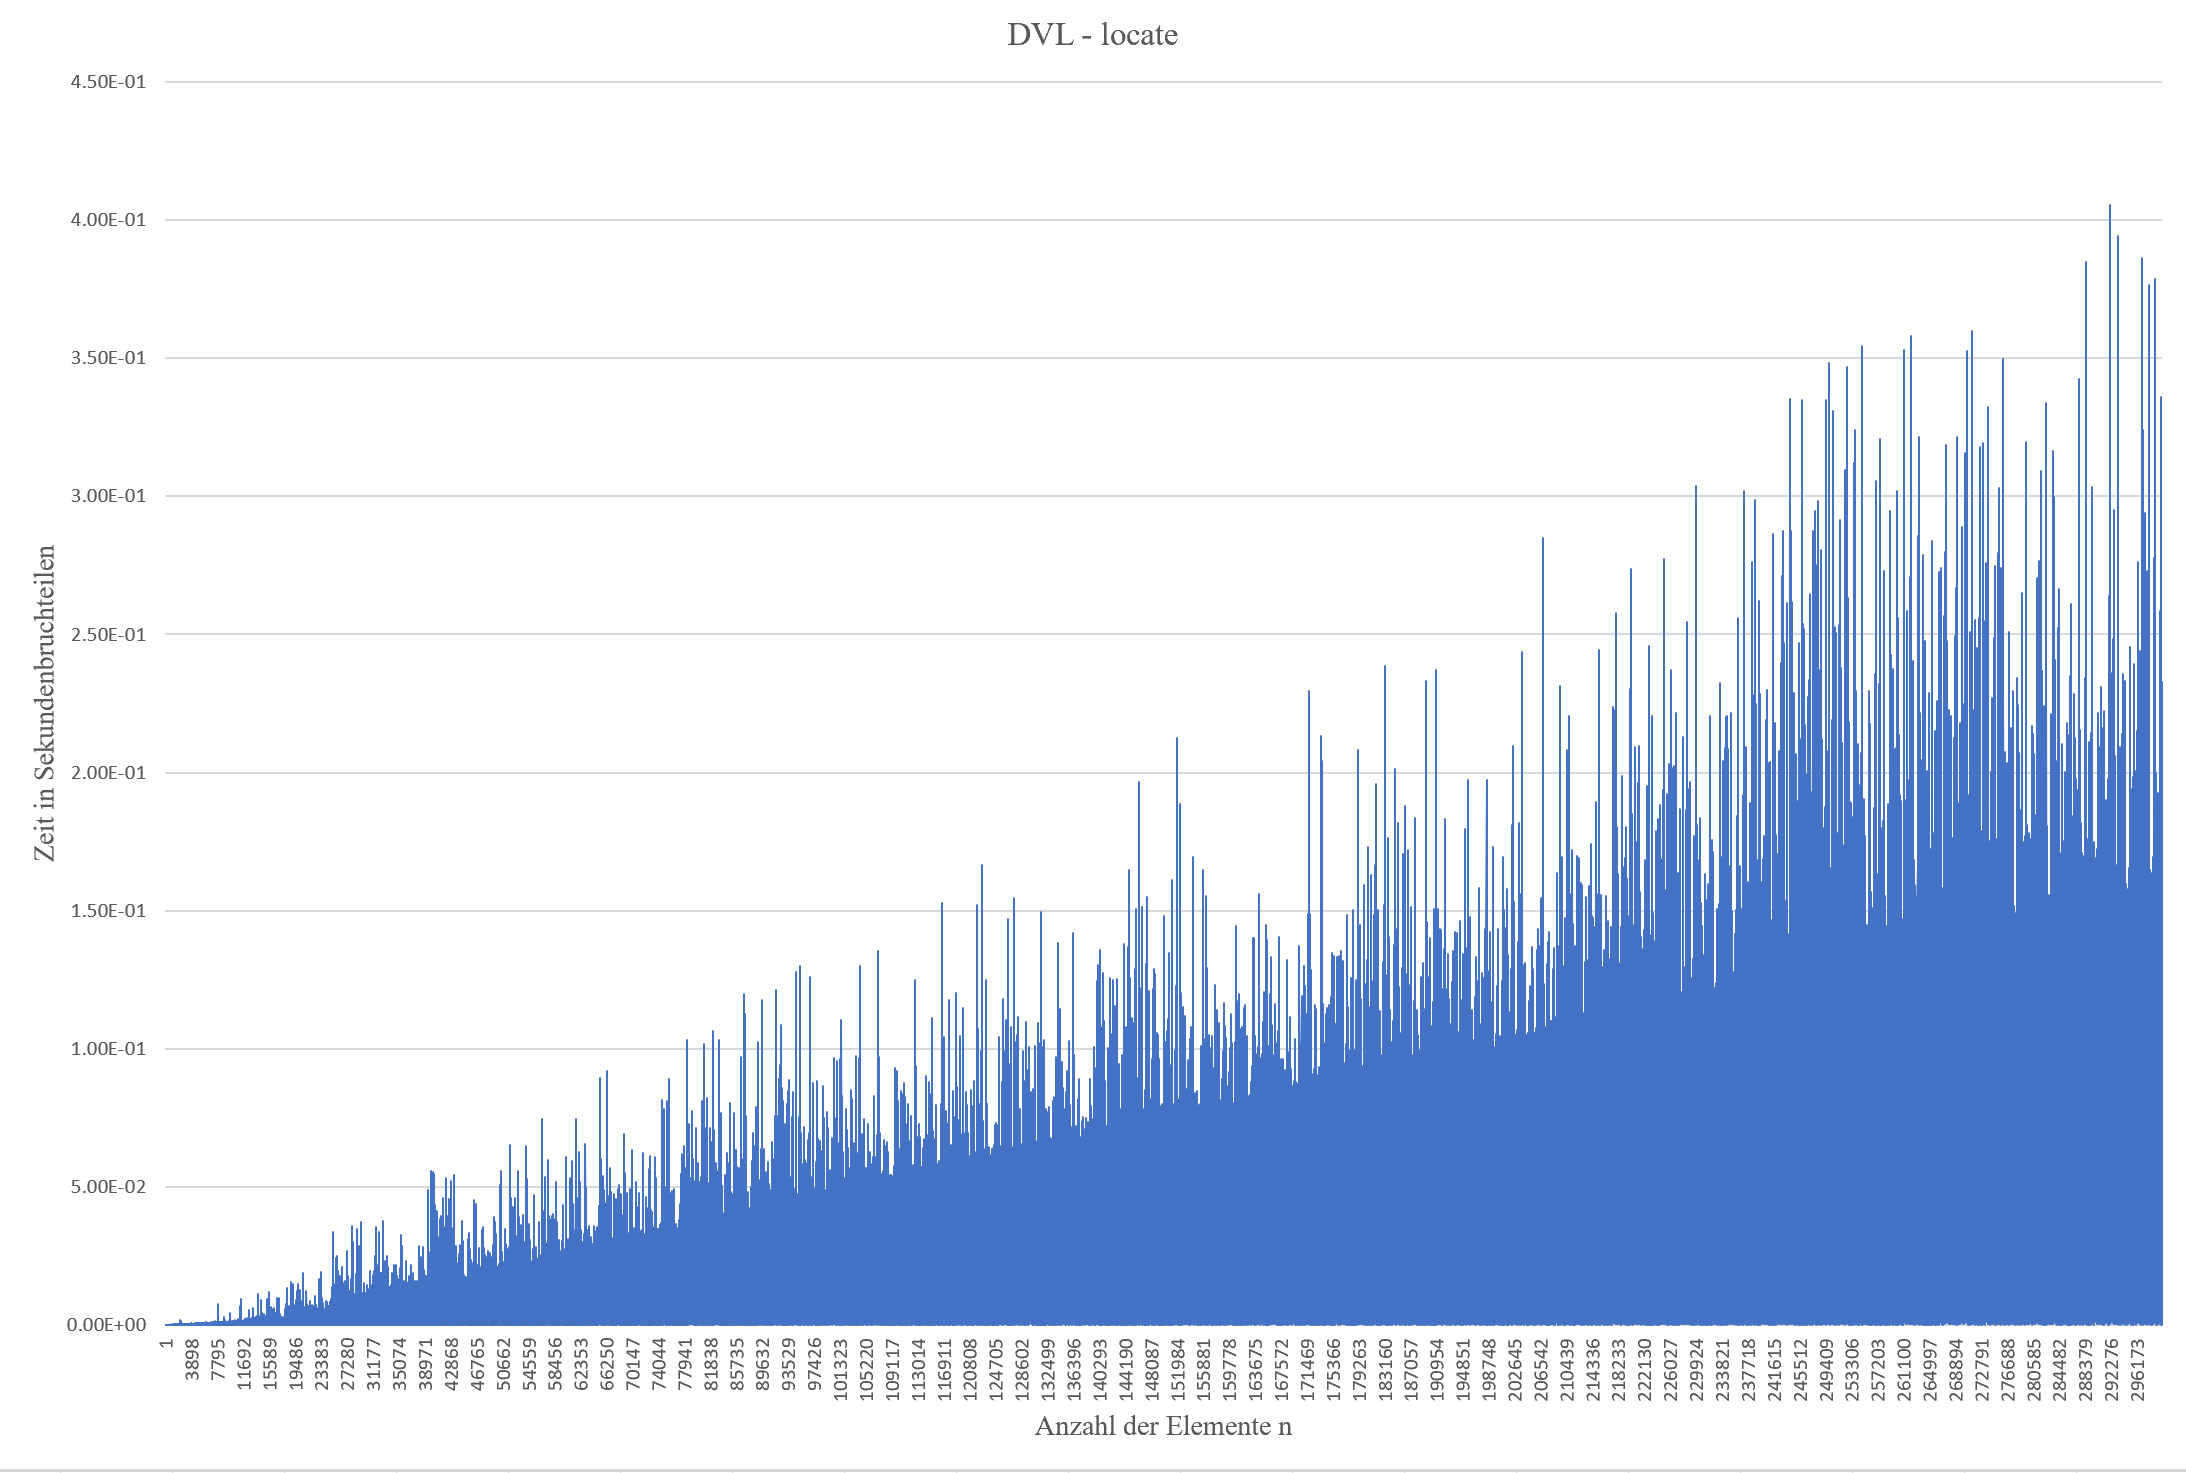
\includegraphics[width=\linewidth]{assets/benchlist.png}
        \caption{Die unbearbeiteten Ergebnisse des Tests an einer Doppelt Verketteten List (DVL) mit maximal 300.000 Elementen. Dargestellt ist die Dauer der Funktion \texttt{locate}. Die Messspitzen lenken hier weniger vom Ergebnis ab als bei (a,b)-Bäumen. Die lineare Laufzeit ist deutlich erkennbar.}
        \label{fig:benchmark10raw}
    }
\end{figure}
